% XCircuit output "full_adder.tex" for LaTeX input from full_adder.eps
\def\putbox#1#2#3#4{\makebox[0in][l]{\makebox[#1][l]{}\raisebox{\baselineskip}[0in][0in]{\raisebox{#2}[0in][0in]{\scalebox{#3}{#4}}}}}
\def\rightbox#1{\makebox[0in][r]{#1}}
\def\centbox#1{\makebox[0in]{#1}}
\def\topbox#1{\raisebox{-0.60\baselineskip}[0in][0in]{#1}}
\def\midbox#1{\raisebox{-0.20\baselineskip}[0in][0in]{#1}}
   \scalebox{1}{
   \normalsize
   \parbox{8.61458in}{
   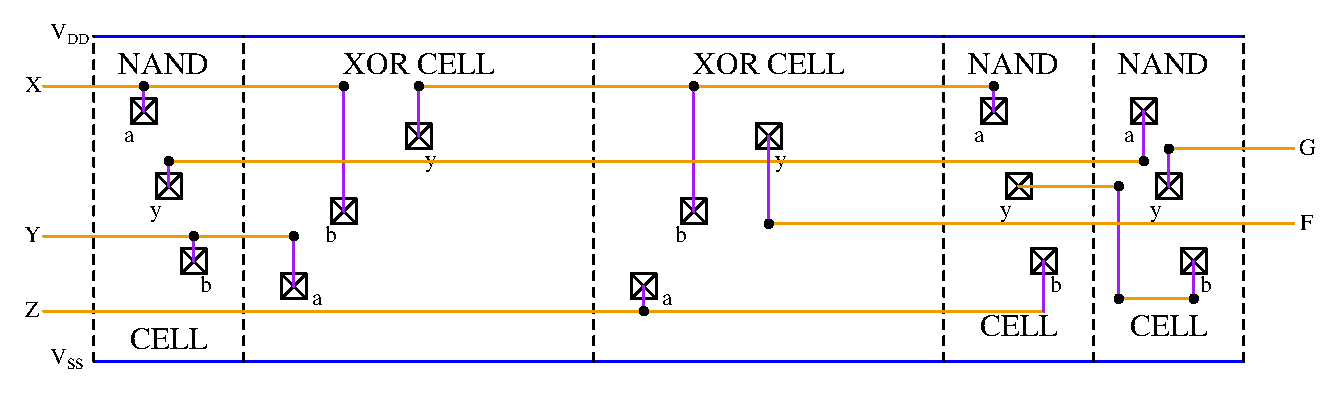
\includegraphics[scale=1]{full_adder.eps}\\
   % translate x=888 y=714 scale 0.38
   \putbox{2.68in}{3.02in}{1.20}{\midbox{123}}%
   \putbox{3.76in}{2.94in}{1.20}{jhgj}%
   } % close 'parbox'
   } % close 'scalebox'
   \vspace{-\baselineskip} % this is not necessary, but looks better
